\documentclass{article}

\usepackage{graphicx} 
\usepackage[colorlinks=true,
            linkcolor=blue,
            citecolor=blue,
            urlcolor=blue,
            ]{hyperref}

\usepackage{graphicx}
\usepackage{amsmath,amssymb}
\usepackage{color}

\newcommand{\coursedir}{http://www.stanford.edu/class/stats191}
\newcommand{\Rdocdir}{http://www-stat.stanford.edu/~jtaylor/R/doc}
\newcommand{\R}{\href{http://cran.r-project.org}{R}}

\renewcommand{\theenumi}{\arabic{enumi}}
\renewcommand{\labelenumi}{Q. \theenumi)}
\renewcommand{\theenumii}{\alph{enumii}}
\renewcommand{\labelenumii}{(\theenumii)}

\newcommand{\homeurl}{http://www-stat.stanford.edu/\string~jtaylo/courses/stats191}

\begin{document}

\title{Statistics 191 \\ Introduction to Regression Analysis and Applied Statistics \\ Practice Exam }
\author{Prof. J.  Taylor}
\date{}
\maketitle 

{\sc You may use your 4 single-sided pages of notes}

{\sc This exam is 14 pages long. There are 4 questions, each worth 10 points.}

\vspace{1in}


{\bf \sc I understand and accept the Stanford University Honor Code.}

\vspace{0.5in}

{\bf \sc Name:} \underline{\hspace{2.5in}}

\vspace{0.5in}

{\bf \sc Signature:} \underline{\hspace{2.5in}}

\vspace{1in}
\begin{center}
\begin{tabular}{|c|p{0.8in}|} \hline
  1 & \\ \hline
  2 & \\ \hline
  3 & \\ \hline
  4 & \\ \hline
  Total & \\ \hline
\end{tabular}
  
\end{center}

\newpage

\begin{enumerate}


\item In order to study the relevance of different fields of study in the job market, the Stanford alumni association followed Stanford graduates in the first few years after
graduation. Students were asked their starting salaries, as well
as which sector (i.e. finance, technology, education) they were employed in.
Within the finance field there were (among others)
(20 Math \& Computational Science (MCS) \& 20 English
graduates). 

\begin{enumerate}
\item The first question the researchers addressed was whether an MCS degree was worth more than a English degree in  finance. 
After entering the data in  {\tt R}, they found the following:
\begin{verbatim}
> t.test(mcs, english, var.equal=T, alternative='greater')

        Two Sample t-test

data:  mcs and english
t = 3.718, df = 38, p-value = 0.0003228
alternative hypothesis: true difference in means is greater than 0
95 percent confidence interval:
 5509.375      Inf
sample estimates:
mean of x mean of y
 69457.52  59377.05
\end{verbatim}
Explain the results in the output above and what conclusions
the researchers can draw.

\newpage

\item A friend of your reads the results of this study and says:
  \begin{quote}
{\em    Wow! If I choose MCS as my major, the probability
I'd earn more than a English grad if we both start in finance is about
$1-3*10^{-4}$!}
  \end{quote}
Do you agree with your friend's statement? Explain.


\vspace{3in}

\item How would you obtain the same results in (a) using the {\tt lm} command in {\tt R}? {\sc Approximately
correct syntax is OK here.}

\vspace{3in}

\end{enumerate}
\newpage 

\item 
The study begun in Q. 1) was continued, expanding to several fields:
education, finance and technology; as well as an additional
degree: electrical engineering.   The means in each group were (after rounding)
\begin{center}
\begin{tabular}{|c|c|c|c|} \hline 
& Education & Finance & Technology \\ \hline
EE & 45000 & 70000 & 80000 \\
MCS & 45000 & 70000 & 65000 \\
English & 50000 & 60000 & 50000 \\ \hline
\end{tabular}
\end{center}

\begin{enumerate}
\item Sketch the {\em interaction plot} for this model, depicting the data in the above table.
From this plot, does the type of degree affect your starting salary? What about the field you begin work in? Are there any interactions? Explain.


\newpage

\item The output below results from fitting this model. What kind of a regression model is it?
\begin{verbatim}
> anova(lm(Salary~Degree*Field))
Analysis of Variance Table

Response: Salary
              Df     Sum Sq   Mean Sq  F value
Degree         2 6.2969e+09 ?????????  ???????
Field          2 1.7624e+10 ?????????  ???????
Degree:Field   4 6.7457e+09 ?????????  ???????
Residuals    171 1.4860e+10 ?????????
---

\end{verbatim}
Make a table that includes all values overwritten with {\tt ?}'s above.
({\sc Don't worry if you don't have a calculator, fractions are fine.}) 


\newpage 
\item How would you compute $p$-values for each entry of the {\tt F value} column if you had {\tt R}? Without explicitly computing $p$-values, do the $F$ statistics support your conclusions in (a)? State the hypothesis that each {\tt F value} is testing. {\sc You can use the fact that, with many degrees of freedom in the denominator, an $F$ statistic has expected value 1 if the null hypothesis is true.}

\end{enumerate}


%\begin{figure}
%  \label{fig1}
%  \centering
%  \resizebox{!}{3.5in}{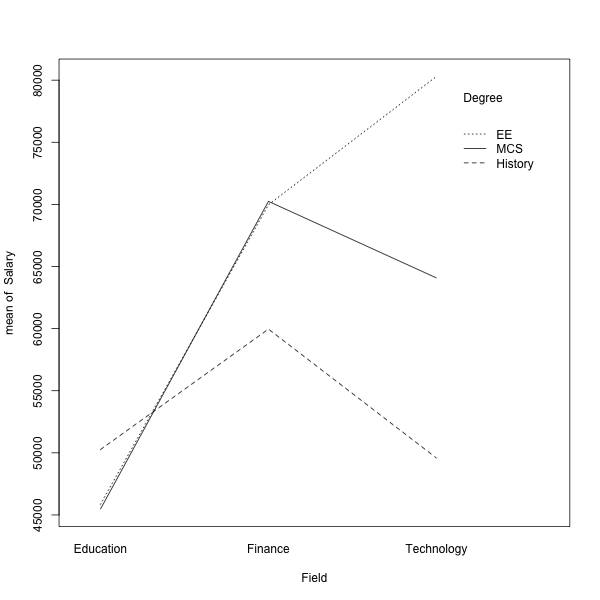
\includegraphics{salary}}
%\caption{Graphic depicting starting salary in three different fields (technology, education, finance) based on three different degrees (history, MCS, EE).}
%\end{figure}


\newpage

\item The incidence of landslides in Northern California increases with the amount of rain that falls in any given year.
 Suppose we are given data of the following form, collected for each month over several years.
 \begin{description}
 \item[ \tt Landslides:] The number of landslide events reported in the Santa Cruz mountains in that specific month.
 \item[ \tt Rainfall:] The average rainfall in the Santa Cruz mountains in that month measured in inches.
 \item[ \tt RainfallP:] The  average rainfall in the Santa Cruz mountains in the previous month measured in inches.
 \end{description}

\begin{enumerate}
\item 
Consider the following {\tt R} output
\begin{quote}
\begin{verbatim}


MA = lm(Landslides ~ Rainfall + RainfallP)
MA
## 
## Call:
## lm(formula = Landslides ~ Rainfall + RainfallP)
## 
## Coefficients:
## (Intercept)     Rainfall    RainfallP  
##      0.6699       0.1065       0.0274
    
MB = glm(Landslides ~ Rainfall + RainfallP, family = poisson())
MB
## 
## Call:  glm(formula = Landslides ~ Rainfall + RainfallP, family = poisson())
## 
## Coefficients:
## (Intercept)     Rainfall    RainfallP  
##      0.1807       0.0414       0.0103  
## 
## Degrees of Freedom: 119 Total (i.e. Null);  117 Residual
## Null Deviance:	    136 
## Residual Deviance: 117 	AIC: 436
    \end{verbatim}
\end{quote}
\newpage

Which model would you think to be the most natural model to model the count of the number of landslide events
in the Santa Cruz mountains? Explain.

\vspace{3in}

\item In whichever model you chose, what is the effect of receiving an additional 10 inches of rain in a given month?

\vspace{3in}

\newpage 
\item How would you use {\tt anova} to test whether the variable {\tt RainfallP} is associated to {\tt Landslides}. 
What is the null hypothesis in your test? The alternative?

\vspace{3in}

\item Suppose you hypothesize that there is a {\em supersaturation} effect.  That is, when rainfall exceeds 15 inches
in a given month, the relationship between {\tt Rainfall} and {\tt Landslides}. You decide to form a variable

\begin{verbatim}
    HeavyRainfall = (Rainfall > 15)
    \end{verbatim}
    
    Write the formula for a model that allows for a different slope and intercept in months of heavy rainfall. How many
    degrees of freedom does this model use to estimate the mean? ({\sc Assume that you have retained the variable {\tt RainfallP} from above.})
    

\end{enumerate}

\newpage


\item A lab scientist is interested in the effect of temperature, $T$ on 
the growth rate of a certain population of bacteria. 
For each of the temperatures in the Table \ref{table1} below, the scientist performs 
a number of experiments, which can be found in the column $N$, and
records the average growth rate (averaged across all experiments of that temperature) in the column ${\tt Gbar}$  of Table \ref{table1}. That is, 30.4 is the average
of growth rates, $G$, from 7 different experiments each conducted
at a temperature of 80.
The scientist is interested in fitting a linear regression model
for the growth rate as a function of $T$.

\begin{table}
  \centering
\begin{tabular}{rrr}
        {\tt Gbar} &   {\tt N} &    {\tt T} \\ \hline
   30.4 &   7 &   80 \\
   32.1 &   4 &   90 \\
   36.2 &   9 &  100 \\
   33.5 &   3 &  110 \\
   38.4 &  11 &  120 \\
\end{tabular}
\caption{Data on averaged growth rate at different temperatures $T$. The
column $Gbar$ is the average of $N$ different experiments at a fixed temperature
$T$.}
\label{table1}
\end{table}


Assume that a simple linear model of the form
\begin{equation}
  \label{eq:model1}
G = \beta_0 + \beta_1 T + \epsilon  
\end{equation}
is appropriate if the actual growth rates were observed (rather
than ${\tt Gbar}$, their averages over the $N$ experiments). That is,
the variance of $\epsilon$ is constant across different values of $T$
and is distributed as $N(0,\sigma^2)$ independently for each experiment.

\begin{enumerate}

\item The quantities ${\tt Gbar}$ are averages over several experiments. 
What is the relationship between the variances  of the ${\tt Gbar}$ entries in Table \ref{table1} and $\sigma^2$ in \eqref{eq:model1}? Is their variance constant
if \eqref{eq:model1} is correct?

\vspace{3in}


\item Your are given a choice between the following 3 outputs from $R$ to
find a confidence interval for the coefficient $\beta_1$ in the model \eqref{eq:model1}.

\begin{quote}
\begin{verbatim}
> # MODEL A
> confint(lm(Gbar~T, growth))
                  2.5 %     97.5 %
(Intercept) -2.45005910 35.8900591
T           -0.01581187  0.3638119
\end{verbatim}
\end{quote}
\begin{quote}
\begin{verbatim}

> # MODEL B
> confint(lm(Gbar~T, growth, weights=growth$N))
                 2.5 %     97.5 %
(Intercept) 0.13407264 31.3517067
T           0.03736585  0.3399493

\end{verbatim}
\end{quote}
\begin{quote}
\begin{verbatim}

> # MODEL C
> confint(lm(Gbar~T, growth, weights=1/growth$N))
                  2.5 %     97.5 %
(Intercept) -1.07474463 40.0286748
T           -0.06427241  0.3443322

\end{verbatim}
\end{quote}

\newpage

Which of the three models above ($A,B$ or $C$) have unbiased estimates of $\beta_1$ if model \eqref{eq:model1} is correct?

\vspace{3in}


\item Which of the three models above ($A,B$ or $C$) have valid confidence intervals
for $\beta_1$ if model \eqref{eq:model1} is correct? If a model has invalid
confidence intervals, what is wrong with the confidence interval?


\end{enumerate}

\end{enumerate}

   \newpage
   {\sc Extra space}

   \newpage
   {\sc Extra space}



\end{document}




\begin{table}[htbp]
  \centering
  \begin{tabular}{ccc} \hline
Variable & Coefficient & SE  \\ \hline
Constant & 4.03 & 3.26  \\
Units & 15.21 & 0.52  \\ \hline
  \end{tabular}
  \caption{Regression Output When $Y$ is Regressed on $X$ for the computer repair data.}
  \label{tab:1}
\end{table}

For this question, use the following table, based on a regression for predicting the 
length of a service call at a computer repair company and the number of units
needing to be repaired. A total of $n=15$ calls were used to fit the model.

Test the following hypotheses at level $\alpha=0.1$.
\begin{enumerate}
\item $H_0: \beta_1=15$ vs. $H_1:\beta_1 \neq 15$

\item $H_0:\beta_1=15$ vs. $H_1:\beta_1 > 15$ 

\item $H_0:\beta_0=0$ vs. $H_1:\beta_0 \neq 0$ 

\item $H_0:\beta_0=5$ vs. $H_1:\beta_0 \neq 5$ 

\end{enumerate}

What are the assumptions you are making? 


\item A study is conducted to investigate the relationship
between LDL cholesterol (low-density lipoprotein), body
weight (W) and gender (G, 1=Male) in a certain population.
The data can be found at
\begin{quote}
\href{\homeurl/data/LDL.table}{\homeurl/data/LDL.table}  
\end{quote}

Answer the following questions, using $\alpha=0.05$ if not specified.
\begin{enumerate}
\item Is there a linear relationship between LDL and weight? 

\item Is the relationship the same within the male and female groups? If not, what is
different?

\item Use a model selection procedure to select a model that best describes the relationship between LDL, weight and gender in this population.
\end{enumerate}


\end{enumerate}



 \item Three types of fertilizer are to be tested to see
which one yields more corn crop. Forty similar plots of land were available
for testing purposes. The 40 plots are divided at random into four groups,
ten plots in each group. Fertilizer 1 was applied to each of the ten corn plots
in Group 1. Similarly, Fertilizers 2 and 3 were applied to the
plots in Groups 2 and 3, respectively. The corn plants in Group 4
were not given any fertilizer; it will serve as the control group.
The data can be found at
\begin{quote}
\href{\homeurl/data/yield.table}{\homeurl/data/yield.table}  
\end{quote}

Answer the following questions, using $\alpha=0.05$ if not specified.
\begin{enumerate}
\item With $Y_{ij}$ being the $j$-th observation in the $i$-th group,
fit a model
$$
Y_{ij} = \mu_i + \varepsilon_{ij}.
$$

\item Test the hypothesis that, on the average, none of the three
types of fertilizer has an effect on corn crops. Specify the hypothesis
to be tested, the test statistic and the results.

\item Test the hypothesis that, on the average, the three
types of fertilizer has the same effect on corn crops but different
than the control group 4. Specify the hypothesis
to be tested, the test statistic and the results.


\item Find Bonferroni simultaneous 90\% confidence intervals for the
mean yield in each of the four groups.
\end{enumerate}


\item 
\begin{table}[htbp]
  \centering
  \begin{tabular}{r|ll} 
&          Df & SSE  \\ \hline
Use &          2 &  33.24 \\
Size  &         3 &  12.06  \\
Size:Use &        6 &   4.25  \\
Residuals & 108 & 154.62 
  \end{tabular}
  \caption{ANOVA output for gasoline consumption analysis}
  \label{tab:3}
\end{table}

In order to determine some of the factors that effect
gasoline consumption, the fuel average miles per gallon for
 120 families and their cars were tracked over several months. The 
cars were categorized in to 4 categories: compact, sedan, minivan, SUV;
and the prevalent use was broken down into 3 categories: commuting to work, weekend, driving to school.
The sums of squares of a two-way analysis of variance (ANOVA)
model are presented above. 

\begin{enumerate}
\item What assumptions does the two-way ANOVA model make? Be as precise as possible.

\item Test for the main effects of both Use and Size at level $\alpha=0.05$.
Does Use and / or  Size have an effect on average MPG?

\item Is there any significant interaction (at level $\alpha=0.05$) between 
Use and Size and their effect on average MPG?
\end{enumerate}

\item 
\begin{table}[htbp]
  \centering
  \begin{tabular}{c|ccccc} \hline
&  Contra Costa & Santa Clara & Los Angeles & San Bernadino \\ \hline
Yes   &  117	& 222 & 	 133 	& 109 	   \\
No &	404  &	334 	& 204  &	263   \\ \hline
  \end{tabular}
  \caption{Responses to earthquake insurance survey for Q. 4)}
  \label{tab:2}
\end{table}

A questionnaire was sent out to California homeowners asking whether or not
they had purchased earthquake insurance.

\begin{enumerate}
\item Test at level $\alpha=0.05$, using a Poisson regression model, whether the probability of having
earthquake insurance is the same in each county in the survey. What assumptions are you making in the model? What is the null hypothesis, $H_0$? The alternative $H_a$?


\item Also of interest is whether the probability of a homeowner having earthquake insurance is 50\% in
all counties. Translate the probability being 50\% into a statement
about the means in the Poisson model.
\item Test the hypothesis, at level $\alpha=0.05$ that the probability of having earthquake insurance is 50\% in each county surveyed.

\end{enumerate}

\item 
Figure 1 shows the data from a regression study
with only one predictor. In each question, the correct answer
may be more than one of
$A,B$ or $C$.
  \begin{figure}
\label{fig1}
    \centering
    \resizebox{!}{4in}{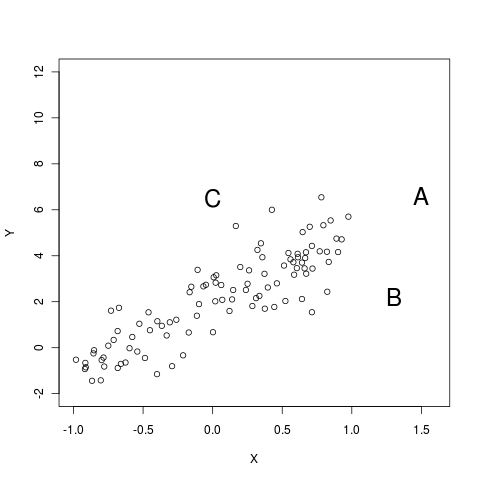
\includegraphics{leverage}}
\caption{Figure for Q. 3)}
  \end{figure}

  \begin{enumerate}
  \item Give a definition of {\em leverage}. 
Which of the labelled points ($A, B$ or $C$)
would you think have a high leverage value? Explain.
%A, B

\item Which of the labelled points ($A, B$ or $C$)
would you think would be labelled as an outlier by an outlier detection test? Explain.
% B or C

\item What does Cook's Distance try to measure for a multiple linear regression model? Which of the labelled points ($A, B$ or $C$)
would you think would have a large Cook's distance? Explain.
  \end{enumerate}
% B or C





\item Suppose we split mammalian species into 5 groups based on a
notion of {\em danger level} {\tt D}. That is, mammals in group 1
are high up on the food chain, while mammals in group 5 are low on the
food chain and must constantly be looking for predators. We would expect
mammals in group 1 can sleep more soundly than mammals in group 5. We might also
suspect that the total hours slept in a day, {\tt TS} is related to metabolic
needs and might be related to the mammals' size as measured by body weight
{\tt BodyWt}. We fit the following four models:

\begin{quote}
\begin{verbatim}
> M1
...
Coefficients:
(Intercept)  log(BodyWt)  
    11.4377      -0.7931  

> M2
...
Coefficients:
(Intercept)  log(BodyWt)           D2           D3           D4           D5  
    13.9325      -0.6287      -2.4287      -3.5836      -3.8535      -7.2945  

> M3
...
Coefficients:
   (Intercept)  log(BodyWt):D1  log(BodyWt):D2  log(BodyWt):D3  log(BodyWt):D4  
       11.6259         -0.2892         -0.5930         -0.9325         -0.6414  
log(BodyWt):D5  
       -1.6585  

> M4
...
Coefficients:
   (Intercept)              D2              D3              D4              D5  
       13.8682         -2.3592         -3.5009         -4.2274         -7.0311  
log(BodyWt):D1  log(BodyWt):D2  log(BodyWt):D3  log(BodyWt):D4  log(BodyWt):D5  
       -0.5810         -0.6155         -0.9254         -0.4114         -0.6774  

> 



\end{verbatim}
\end{quote}

\begin{enumerate}
\item Which model of {\tt M1,M2,M3,M4} assumes that the relationship
between {\tt log(BodyWt)} and {\tt TS} is the same within each level of 
{\tt D}?

\vspace{0.3in}   

\item Which model of {\tt M1,M2,M3,M4} allows for the relationship
between {\tt log(BodyWt)} and {\tt TS} to have a different intercept for each level of 
{\tt D}?

\vspace{0.3in}   

\item Which model of {\tt M1,M2,M3,M4} allows for the relationship
between {\tt log(BodyWt)} and {\tt TS} to have a different slope for each level of 
{\tt D}?

\vspace{0.3in}   

\item Which model of {\tt M1,M2,M3,M4} allows for the relationship
between {\tt log(BodyWt)} and {\tt TS} to have both a different intercept and slope for each level of {\tt D}?

\vspace{0.3in}   


\item Figure 4 is a plot of {\tt log(BodyWt)} vs. {\tt TS} 
with the `1's representing those for which {\tt D==1}, etc, while
Figure 5 has regression lines, fit within groups separately, added to the plot. Based on this plot which model do you think is most appropriate? Explain.

\newpage

\item Does your model from (e) agree with the following output? Explain.

  \begin{quote}
\begin{verbatim}
> anova(M1,M4)
Analysis of Variance Table

Model 1: TS ~ log(BodyWt)
Model 2: TS ~ log(BodyWt):D + D
  Res.Df    RSS Df Sum of Sq      F   Pr(>F)   
1     56 866.23                                
2     48 565.46  8    300.77 3.1915 0.005532 **
---
Signif. codes:  0 ‘***’ 0.001 ‘**’ 0.01 ‘*’ 0.05 ‘.’ 0.1 ‘ ’ 1 
> anova(M2,M4)
Analysis of Variance Table

Model 1: TS ~ log(BodyWt) + D
Model 2: TS ~ log(BodyWt):D + D
  Res.Df    RSS Df Sum of Sq      F Pr(>F)
1     52 581.22                           
2     48 565.46  4    15.760 0.3345 0.8534
> anova(M3,M4)
Analysis of Variance Table

Model 1: TS ~ log(BodyWt):D
Model 2: TS ~ log(BodyWt):D + D
  Res.Df    RSS Df Sum of Sq      F  Pr(>F)  
1     52 709.49                              
2     48 565.46  4    144.04 3.0567 0.02533 *
---
Signif. codes:  0 ‘***’ 0.001 ‘**’ 0.01 ‘*’ 0.05 ‘.’ 0.1 ‘ ’ 1 
> 

\end{verbatim}
  \end{quote}

  \begin{figure}
\label{fig4}
    \centering
    \resizebox{!}{3in}{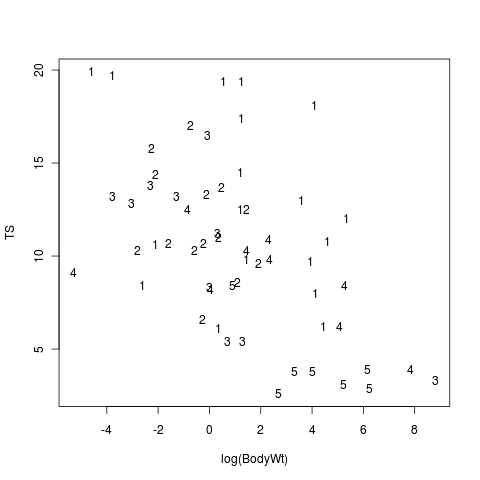
\includegraphics{sleep}}
\caption{{\tt log(BodyWt)} vs. {\tt TS} for Q. 3)}
  \end{figure}

  \begin{figure}
\label{fig5}
    \centering
    \resizebox{!}{3in}{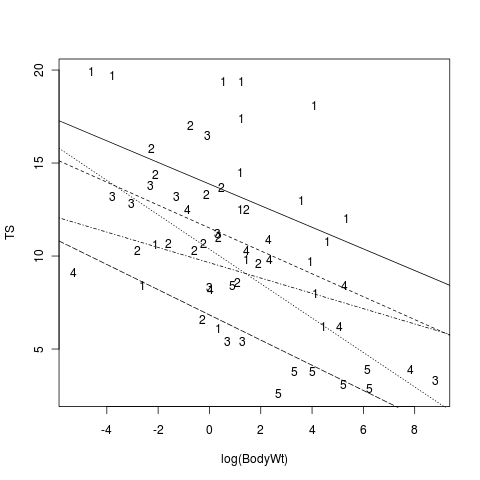
\includegraphics{sleep_fit}}
\caption{{\tt log(BodyWt)} vs. {\tt TS} for Q. 3)}
  \end{figure}

  \end{enumerate}


\newpage

\item Apple is one of the most highly valued companies in the world
and may be expected to have some effect on other technology stocks. You decide to investigate this hypothesis using
daily close of the NASDAQ 100 (symbol {\tt QQQ}) as a function of the 
{\tt AAPL} daily close price for all 252 trading days in the year 2011. 
Instead of directly modelling the price, we use the daily returns, as
suggested by the random walk model of stock prices:

\begin{quote}
\begin{verbatim}

> QQQr = QQQ[2:252]-QQQ[1:251]
> AAPLr = AAPL[2:252]-AAPL[1:251]

\end{verbatim}
\end{quote}

\begin{enumerate}
\item Consider the following output
  \begin{quote}
\begin{verbatim}
> summary(lm(QQQr~AAPLr))
...
Residuals:
     Min       1Q   Median       3Q      Max 
-1.45411 -0.27126 -0.02026  0.34650  1.30207 

Coefficients:
            Estimate Std. Error t value Pr(>|t|)    
(Intercept) 0.030293   0.031336   0.967    0.335    
AAPLr       0.107698   0.005151  20.906   <2e-16 ***
---
Signif. codes:  0 ‘***’ 0.001 ‘**’ 0.01 ‘*’ 0.05 ‘.’ 0.1 ‘ ’ 1 

Residual standard error: 0.4959 on 249 degrees of freedom
Multiple R-squared: 0.6371,	Adjusted R-squared: 0.6356 
F-statistic: 437.1 on 1 and 249 DF,  p-value: < 2.2e-16 

\end{verbatim}
  \end{quote}
Does this model support the hypothesis that 
{\tt AAPL} is highly correlated with the {\tt QQQ} price? How much of the overall variability of
the returns of {\tt QQQ} are explained by the returns of {\tt AAPL}?

\newpage

\item Figure 6 shows the residuals from the above model
plotted in time, while Figure 7 shows the estimated
autocorrelation function of the residuals. Does this suggest
you should modify the previous model?

\vspace{1in}

  \begin{figure}
\label{fig6}
    \centering
    \resizebox{!}{3in}{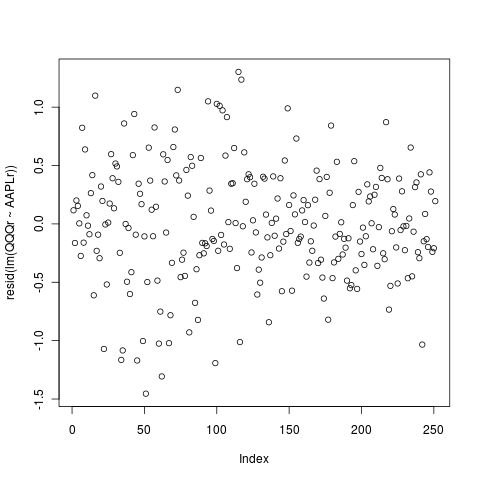
\includegraphics{stock_resid}}
\caption{Residuals of {\tt lm(QQQr\string~AAPLr)}.}
  \end{figure}

  \begin{figure}
\label{fig7}
    \centering
    \resizebox{!}{3in}{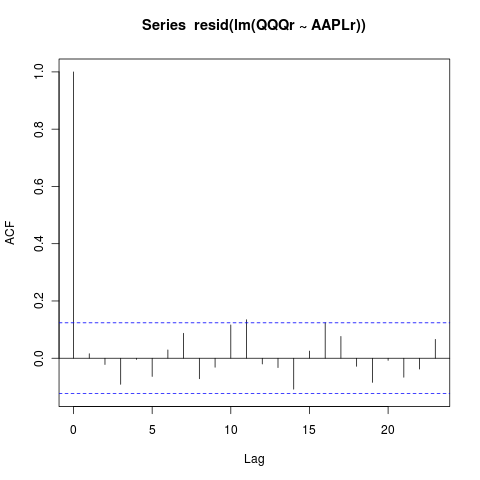
\includegraphics{stock_acf}}
\caption{Residuals of {\tt lm(QQQr\string~AAPLr)}.}
  \end{figure}

\item What can we conclude from the following output:

  \begin{quote}
\begin{verbatim}
> durbinWatsonTest(lm(QQQr~AAPLr))
 lag Autocorrelation D-W Statistic p-value
   1      0.01594918      1.967258   0.848
 Alternative hypothesis: rho != 0
\end{verbatim}

  \end{quote}

\newpage

\item Suppose the autocorrelation in (c) is far from 0. How could we modify the regression model to account for this autocorrelation. If the autocorrelation was not zero and we did not modify our model, what can we reliably say about the
model {\tt lm(QQQr \string ~AAPLr)}? Be as specific as possible.

\vspace{1in}


\end{enumerate}

\end{enumerate}




